\documentclass[11pt,fullpage]{book}
\title{\textbf{~~~~~~~~~~~~~~~}\newline Bayesian book}
\author{}
\usepackage{natbib}
\usepackage{url,times}
\usepackage{graphicx}
\usepackage{epstopdf}
\usepackage{amsmath}
\usepackage[all]{xy}
\usepackage{pxfonts}
\usepackage{colortbl}
\usepackage{color}
\usepackage{subfigure}
\usepackage{gensymb}
\usepackage{ctable}
\usepackage[justification=centering]{caption}[2007/12/23]
\usepackage{longtable}
\usepackage{pstricks-add}
\usepackage{pstricks}
\usepackage{pst-func}
\usepackage{pst-math}

\setlength{\parindent}{0.0in}
\setlength{\parskip}{0.1in}
\maketitle

\begin{document}
\tableofcontents
\chapter{How to best use this book}
\part{Understanding the Bayesian formula}
\chapter{The subjective worlds of frequentist and Bayesian statistics}

\chapter{Likelihoods}\label{chap:Likelihoods}
\section{Chapter Mission statement}
At the end of this chapter a reader will know how to choose an appropriate likelihood model for most situations. Further the reader will understand the basis behind maximum likelihood estimation.

Insert a graphic with the likelihood part of Bayes' formula circled, as in the equation shown below for the part highlighted in blue.

\begin{equation}
P(\theta|data) = \frac{{\color{blue}P(data|\theta)}\times P(\theta)}{P(data)}
\end{equation}\label{eq:Likelihood_BayesHighlighted}

\section{Chapter goals}
The starting point of the right hand side of the Bayesian formula is the likelihood function. This chapter will explain what is meant by a likelihood function, and why it is incorrect to view it as a probability for Bayesians. Further the choice over which likelihood to use for a given situation is often difficult to those unfamiliar with statistics. This chapter will provide practical guidance to likelihood choice, which should allow the student to be confident in their choice of model. As an important stepping stone to Bayesian estimation, this chapter will also explain how classical maximum likelihood estimation works. 

\section{What is a likelihood?}
In all statistical inference, we use an idealised, simplified, model to try to mimic relationships between real variables of interest. This model is then used to test hypotheses about the nature of the relationships between these variables. In Bayesian statistics the evidence for a particular hypothesis is summarised in posterior probability distributions. Bayes' magic rule tells us how we can compute this posterior probability distribution for a given parameter within a model, $\theta$:

\begin{equation}
P(\theta|data) = \frac{P(data|\theta)\times P(\theta)}{P(data)}
\end{equation}\label{eq:Likelihood_Bayes}

The first step to understanding this formula (so that we can ultimately use it!) is to understand what is meant by the numerator term, $P(data|\theta)$, which Bayesians call a Likelihood! Firstly, it's important to say that what we really mean by the numerator is:

\begin{equation}
P(data|\theta) = Probability(data|\theta,Model \; Choice)
\end{equation}\label{eq:Likelihood_simple}

What (\ref{eq:Likelihood_simple}) means is, what is the probability that we would have obtained the 'data', given (this is represented by the $|$ symbol) a particular value of $\theta$ and a particular choice of model. In other words, if our statistical model were true, and the value of the model's parameter were $\theta$, (\ref{eq:Likelihood_simple}) tells us the probability that we would have obtained our data. 

But what does this mean in simple, everyday language? Imagine that we flip a \textit{fair} coin. The most simple statistical model for coin flipping we can pick is to disregard the angle it was thrown at, as well as its height above the surface, along with any other details, and just pick the probability of the coin coming heads to be $\theta=\frac{1}{2}$. Furthermore, if a coin is thrown twice, we might choose to model the situation by assuming that the throwing technique is sufficiently similar between the two throws such that we can model each throw as independently having a probability of $\frac{1}{2}$. It's important to note that it is an assumption to forget about the throwing angle, as well as height of throw for each throw, and this forms part of our model of the situation. In this idealised model\footnote{Albeit in practicality, this is a pretty reasonable representation of the situation for most purposes.} of the situation the probability of the coin coming up as heads twice is simply $\frac{1}{2}\times\frac{1}{2}=\frac{1}{4}$. Written mathematically, this is simply the likelihood:

\begin{equation}
P(HH|\theta=\frac{1}{2},Simple\;Model) = \frac{1}{4}
\end{equation}\label{eq:Likelihood_fairCoin}

Hence, the likelihood simply summarises the possibility of obtaining a given set of data given a choice of model \textit{and} choice of the model's parameter(s). If we continue to assume that the probability of a head, $\theta$, is given by $\frac{1}{2}$, we can calculate the corresponding probabilities for all outcomes of throwing the coin twice. The most heads that can show up is 2, and the least being zero (if both flips come up tails). Figure \ref{fig:Likelihood_fairCoin} displays the probabilities for this model of the situation. The most likely number of heads to occur is 1, since this can occur in two different ways - either the first coin comes up heads, and the second is tails, or vice versa - whereas the other possibilities (all heads, or no heads) can each only occur in one way. The important thing to note however about figure \ref{fig:Likelihood_fairCoin} isn't the individual probabilities, it is that it represents as a whole a \textit{proper} probability distribution. What do we mean by this? Well, the individual event probabilities are all greater than 0 and less than 1, and when we sum the individual probabilities together we get 1 overall. So in the case where we assume a particular value for $\theta$, and keep it fixed there, the likelihood really is simply just a probability distribution. So, why do we bother changing its names from a 'probability' to a 'likelihood'? That is to be explained in the next section...

\begin{figure}
\centering
\scalebox{0.25} 
{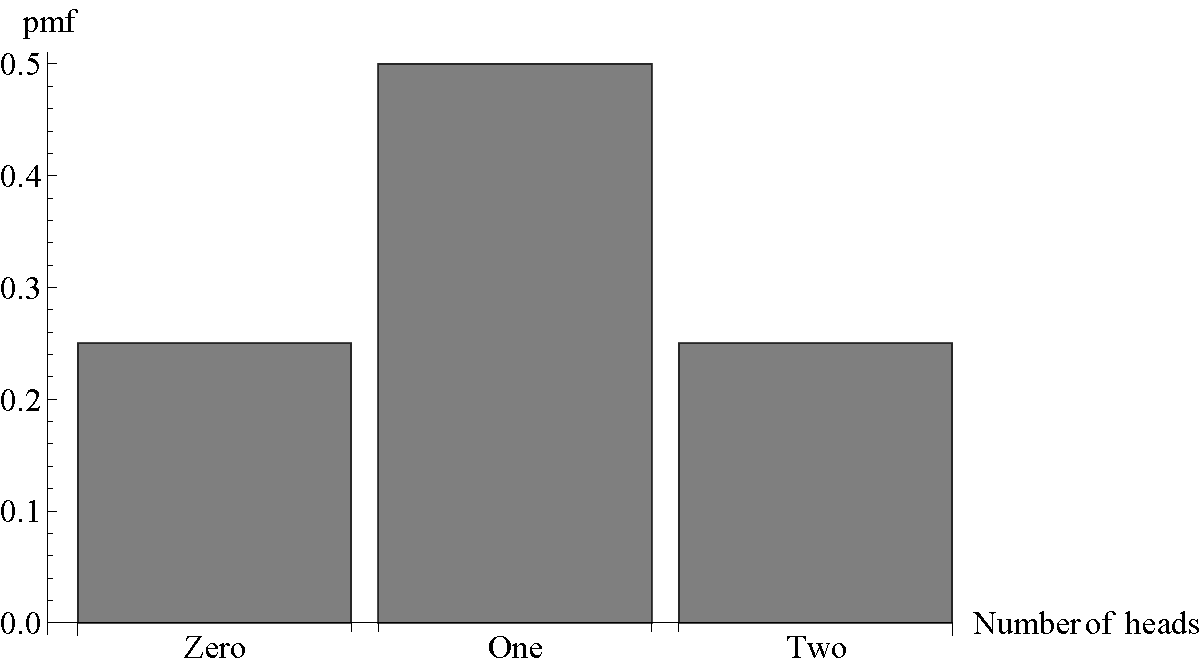
\includegraphics{Likelihood_fairCoin.png}}
\caption{Insert bar chart here of the number of heads along the x axis - 0,1,2 - and the associated probability of each of these outcomes as being the bar height - (1/4,1/2,1/4).}\label{fig:Likelihood_fairCoin}
\end{figure}

\section{Why is a likelihood not a probability for Bayesians?}
When we hold the parameters of our model fixed, as when we held the probability of an individual throw turning up heads to be $\theta=\frac{1}{2}$, we've reasoned that the first term of the numerator of Bayes' rule in (\ref{eq:Likelihood_Bayes}) really is simply a probability. So why don't we just keep calling it that, and forgo the introduction of this new word 'likelihood'? 

The reason is that in Bayesian inference, we \textit{don't} keep the parameters of our model fixed! In Bayesian analysis, it is the \textit{data} that is fixed, and we vary the parameters. Why do we do this? It is because a posterior probability distribution is a probability of a parameter in a model taking on a particular value, across a range of different parameter values. For the case of a coin, where we don't know the probability of a head beforehand, what we hope to get out is a probability distribution of the kind shown in figure \ref{fig:Likelihood_posteriorExample}. Notice that the x-axis in figure \ref{fig:Likelihood_posteriorExample} is the value of $\theta$ - the probability of a heads being obtained. In order to get this posterior probability, $P(\theta|data)$, for each value of theta, we use Bayes' rule in (\ref{eq:Likelihood_Bayes}). This means that for each \textit{different} value of $\theta$, we calculate the first part of the numerator which is $P(data|\theta)$; meaning that we calculate this across a range of $\theta$. If we assume that we have obtained two heads, and vary $\theta$ between 0 and 1 we can obtain the likelihood, which is shown in figure \ref{fig:Likelihood_coinLikelihood}. On first glances in might appear like \ref{fig:Likelihood_coinLikelihood} is a probability distribution, but first looks can be deceiving. 

\begin{figure}
\centering
\scalebox{0.25} 
{\includegraphics{Likelihood_posterior example.png}}
\caption{An example posterior distribution for the probability of a heads.}\label{fig:Likelihood_posteriorExample}
\end{figure}

\begin{figure}
\centering
\scalebox{0.25} 
{\includegraphics{Likelihood_likelihood.png}}
\caption{The x-axis here is theta, ranging between 0 and 1, assuming that one head is obtained this graphs the likelihood, which does not sum to 1.}\label{fig:Likelihood_coinLikelihood}
\end{figure}

Checking off our necessary components of a probability distribution, we first note that all the values of the distribution in figure \ref{fig:Likelihood_coinLikelihood} are non-negative; which is what we require. However, if we look at the area underneath the curve in figure \ref{fig:Likelihood_coinLikelihood}, we find that it does not integrate to 1! Thus we have a violation of the second condition for a valid probability distribution. Hence, when we vary $\theta$ we find that, $P(data|\theta)$ is not a valid probability distribution! We thus introduce the term 'likelihood' to represent value of $P(data|\theta)$ when we vary the parameter, $\theta$. Often the following notation is used to emphasise that likelihood is a function of the parameter $\theta$ with the data held fixed:

\begin{equation}
\mathcal{L}(\theta|data) = P(data|\theta)
\end{equation}\label{eq:Likelihood_notation}

However, in this book, we will persist with the original notation as this is most typical in the literature, under the implicit assumption that when we vary the parameters in question, the term is not strictly a probability.

To provide further justification for this argument, consider the following (albeit contrived) example. Suppose that, we throw a coin twice, and we are told beforehand that the probability of obtaining a head on a particular throw is one of six discrete values: $\theta\in\{0.0,0.2,0.4,0.6,0.8,1.0\}$. In this circumstance, we can calculate the probability of the number of heads, $X$, occurring as:

\begin{align}\label{eq:Likelihood_OneHead}
P(X = 0|\theta)& = P(TT|\theta) = P(T|\theta)\times P(T|\theta) = (1-\theta)^2\\
P(X = 1|\theta)& = P(HT|\theta) + P(TH|\theta) = 2\times P(T|\theta)\times P(H|\theta) = 2\theta(1-\theta)\\\label{eq:Likelihood_TwoHead}
P(X = 2|\theta)& = P(HH|\theta) = P(H|\theta)\times P(H|\theta) = \theta^2
\end{align}

In (\ref{eq:Likelihood_OneHead}), the probability is simply given by the product of the probabilities of not obtaining a head on the first throw, $(1-\theta)$, by the probability of not obtaining a head in the second\footnote{Since we have assumed a model whereby the results of the first and second throws are independent, conditional on $\theta$. In other words, all the similarity between the two throws is captured in the parameter $\theta$.}, which is also $(1-\theta)$. The factor of two arises in (\ref{eq:Likelihood_TwoHead}) since there are two ways of getting one head: \{HT,TH\}.

We can represent the corresponding values of likelihood/probability as in table \ref{tab:Likeihood_BayesBox}. In this form we can see the impact of varying the data (moving along each row), and contrast it with the effect of varying $\theta$ (moving down each column). The important thing to see here is that if we hold the parameter fixed - regardless of this initial choice of $\theta$ - and move along each row summing the entries, we find that the values sum to 1; meaning that this is a proper probability distribution. By contrast, when we hold the number of heads fixed, and vary the parameter $\theta$, moving down each column, summing the entries, we find that the values do not sum to 1. Hence, when we vary $\theta$, we are not dealing with a proper probability distribution, thus meriting the use of the term 'likelihood'.

In Bayesian inference, we always vary the parameter, and implicitly hold the data fixed. Thus, from a Bayesian perspective it is important to use the term Likelihood to indicate that we recognise we are not dealing with a probability distribution.


\begin{table}[htbp]
  \centering
  
    \begin{tabular}{ccccc}
    \multicolumn{5}{c}{\textbf{Number of heads}} \\
    \midrule
    \textbf{$\theta$} & \multicolumn{1}{c}{\textbf{0}} & \multicolumn{1}{c}{\textbf{1}} & \multicolumn{1}{c}{\textbf{2}} &  \multicolumn{1}{c}{\textbf{Total}} \\
    \hline
    \textbf{0.0} & \multicolumn{1}{c}{1.00} & \multicolumn{1}{c}{0.00} & \multicolumn{1}{c}{0.00} & \multicolumn{1}{c}{\textbf{1.00}} \\
    \textbf{0.2} & \multicolumn{1}{c}{0.64} & \multicolumn{1}{c}{0.32} & \multicolumn{1}{c}{0.04} & \multicolumn{1}{c}{\textbf{1.00}} \\
    \textbf{0.4} & \multicolumn{1}{c}{0.36} & \multicolumn{1}{c}{0.48} & \multicolumn{1}{c}{0.16} & \multicolumn{1}{c}{\textbf{1.00}} \\
    \textbf{0.6} & \multicolumn{1}{c}{0.16} & \multicolumn{1}{c}{0.48} & \multicolumn{1}{c}{0.36} & \multicolumn{1}{c}{\textbf{1.00}} \\
    \textbf{0.8} & \multicolumn{1}{c}{0.04} & \multicolumn{1}{c}{0.32} & \multicolumn{1}{c}{0.64} & \multicolumn{1}{c}{\textbf{1.00}} \\
    \textbf{1.0} & \multicolumn{1}{c}{0.00} & \multicolumn{1}{c}{0.00} & \multicolumn{1}{c}{1.00} & \multicolumn{1}{c}{\textbf{1.00}} \\
    \bottomrule
    \textbf{Total} & \multicolumn{1}{c}{\textbf{1.20}} & \multicolumn{1}{c}{\textbf{1.60}} & \multicolumn{1}{c}{\textbf{2.20}} &  \\
    
    \end{tabular}%
  %
  \caption{The values of likelihood for the case of tossing a coin twice, where the probability of heads is constrained to take on a discrete value: \{0.0,0.2,0.4,0.6,0.8,1.0\}. In each of the rows, the value of $theta$ is held constant, meaning that $P(data|\theta)$ is a proper probability distribution and thus the probabilities sum to 1. However, in the columns, the data - the number of heads thrown - is held constant, and thus the probabilities do not sum to 1, and we thus we are better off viewing these data as likelihoods, since they do not satisfy the properties of a proper probability distribution.}\label{tab:Likeihood_BayesBox}
\end{table}

\section{What are models, and why do we need them?}
All models are wrong. They are idealised representations of reality resultant from making assumptions, which if reasonable, may emulate some of the behaviour of a system of interest. Joshua Epstein in an article titled, 'Why model?' emphasises that we perennially build \textit{implicit} mental models for various phenomena \cite{epstein2008model}. Before we go to bed at night we set our alarms for the next morning on the basis of a model. We imagine an idealised - model - morning when it takes us 15 minutes to wake up as a result of an alarm. We use this model to predict how long it will take us to rise from bed, shower, and get changed into clothes in sufficient time to get to work. Whenever we go to the Doctor, they use an internalised biological model of the human body to advise on the best course of treatment for a particular ailment. Whenever we hear expert opinions on TV about the outcome of an upcoming election, the pundits are using mental models of society to explain the results of current polls, as well as make forecasts. As is the case with all models, some of these models are better than others. Hopefully, the models a Doctor uses to prescribe medicine are subject to less error than the opinions of pundits seen on TV! 

Epstein goes on to emphasise that the question, 'Why model?' really means why should we build an \textit{explicit} - written down - model of a phenomena? The point being that \textit{implicit} models are by their very nature, opaque, and not subject to the sort of interrogation and calibration that can be obtained by writing the model on paper. 

We can also ask more narrowly, what are we hoping to gain by building an \textit{explicit} model of a situation? Epstein goes on to suggest 16 reasons, other than prediction, to build a model, of which I list a selected few below:

\begin{itemize}
\item Explain
\item Guide data collection
\item Discover new questions
\item Bound outcomes to plausible ranges
\item Illuminate uncertainties
\item Challenge the robustness of prevailing theory through perturbations
\item Reveal the apparently simple (complex) to be complex (simple) 
\end{itemize}

There are of course other reasons to build models, but I believe that this list encapsulates the majority of them. However, we should not think of this list as static. Whenever we build a model, whether it is statistical, biological or sociological, we should ask, 'What are we hoping to gain by building this model, and how can I judge its success?'. Only when we have a grasp on the answers to these basic questions should we proceed to model building.

\section{How to choose an appropriate model for likelihood?}\label{sec:chooseLikelihood}
Bayesians are acutely aware that their models are wrong. At best, they represent an abstraction from reality, and at worst, they can provide very misleading descriptions of a real phenomenon. Before we use a model for prediction, we should always require that a model is capable of \textit{explanation} of the past and present. With this in mind, I propose the following course of action to specifying a statistical model of which likelihood forms a core part.

\begin{enumerate}
\item Write down the real life behaviour/data patterns that your model should be capable of explaining.
\item Write down the assumptions that we believe are reasonable in order to arrive at such a model.
\item Search for an appropriate/similar model in the literature.
\item Test your model's ability to explain said behaviour/data patterns. If unsuccessful go back to the second step and re-evaluate the appropriateness of your assumptions.
\end{enumerate}

Whilst this methodology is useful for building a statistical model in general, it is more applicable for use with a full Bayesian model, resulting in a posterior distribution. In which case how do we go about specifying a likelihood for a given situation? To answer this we will start with going through a simple example.

\subsection{A likelihood model for an individual's disease status}\label{sec:Likelihood_individualDisease}
Suppose we work for the NHS and we want to build a simple statistical model which is used to explain the prevalence of a certain disease within a sample, which can then be used to make inferences about the population incidence. Also, (unrealistically) let's assume that we start off by assuming that we have a sample of only one person, of which we have no prior information. Let the disease status of that individual be denoted by the variable $X$ which takes on the following binary outcome values dependent on the disease status the individual:

\begin{equation}
X =
\begin{cases}
O & , No\; disease \\
1 & , Positive \; diagnosis
\end{cases}
\end{equation}

The goal of a likelihood model which we specify is to be able to explain probabilistically the relative likelihood that an individual has a disease, as well as make predictions about disease incidence in new samples of individuals. We might assume that a fraction $\theta$ of the population has the disease, and that this individual has come from that population. For each possible outcome, we can use this simple model to specify the probability of each outcome:

\begin{align}\label{eq:Likelihood_SimpleModel1}
P(X = 0|\theta)& = (1-\theta)\\
P(X = 1|\theta)& = \theta\label{eq:Likelihood_SimpleModel2}
\end{align}

However, we would like to be able to write down a single rule which yields (\ref{eq:Likelihood_SimpleModel1}) or (\ref{eq:Likelihood_SimpleModel2}) respectively, dependent on whether $X=0$ or $X=1$ respectively. It transpires that we can do this via the following rule:

\begin{equation}\label{eq:Likelihood_bernoulli}
P(X=\alpha|\theta) = \theta^\alpha(1-\theta)^{1-\alpha}
\end{equation}

Note that in (\ref{eq:Likelihood_bernoulli}) that $\alpha\in\{0,1\}$ refers to the numeric value taken by the variable $X$. The function given in (\ref{eq:Likelihood_bernoulli}) is known as a Bernoulli probability density.

Although this rule for calculating a probability of obtaining a disease status of value $\alpha$ at first looks relatively complex, we see that it reduces to (\ref{eq:Likelihood_SimpleModel1}) and (\ref{eq:Likelihood_SimpleModel2}) if the individual doesn't or does have the disease respectively:

\begin{align}\label{eq:Likelihood_SimpleModel3}
P(X = 0|\theta)& = \theta^0(1-\theta)^1 = (1-\theta)\\
P(X = 1|\theta)& = \theta^1(1-\theta)^0 = \theta\label{eq:Likelihood_SimpleModel4}
\end{align}

Since (\ref{eq:Likelihood_bernoulli}) yields the probability of obtaining any possible value of data, for a given $\theta$, we conclude that this expression is the likelihood. However, we need to be careful, strictly this expression is only a likelihood if we hold the data fixed and vary the parameter $\theta$. Figure \ref{fig:Likelihood_bernoulli} shows that for a fixed value of $theta$ the sum (here we mean the vertical sum) of the two probability densities is always equal to 1. However, when we hold the data fixed, (therefore choosing either the red or green line), we find that the sum of likelihoods across values of $theta$ does not in general equal 1; again demonstrating that when varying parameters that likelihood is not a valid probability density.

\begin{figure}
\centering
\scalebox{0.75} 
{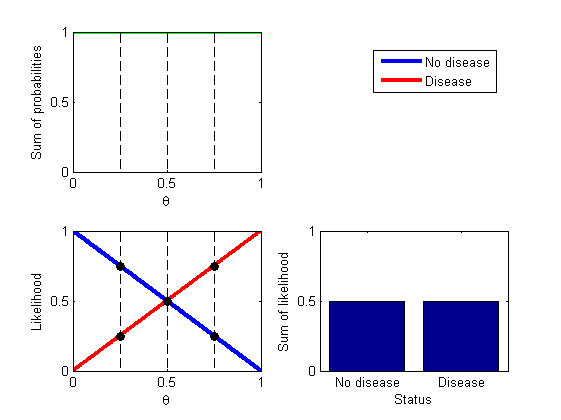
\includegraphics{likelihood_bernoulli.png}}
\caption{The likelihood function as theta varies for the case of the two possible data. For a fixed value of $\theta$ we find that the sum across the values of the probability is always 1. This is because when viewed in this way, the likelihood is really a discrete probability density across the two values which x can take on. However, when we hold the data fixed (choose either the red or blue line) and sum the likelihood horizontally across the values of $theta$ we do not find that the sum is generally equal to 1. }\label{fig:Likelihood_bernoulli}
\end{figure}

\subsection{A likelihood model for disease prevalence of a group}\label{sec:Likelihood_diseaseGroup}
Now we imagine that instead of this solitary individual, we have a group of $N$ individuals. What we would like to do is to calculate the develop a model which will tell us the probability of obtaining $Z$ disease cases within our sample. We would also like to be able to use our model to predict the most likely number of individuals who have the disease in a sample, for a given value of the parameters\footnote{We are starting off by assuming that we know the parameters. Later in this chapter we will obtain a point estimate of the parameters using \textit{Maximum likelihood} estimation.}. 

In order to write down an idealised model we first of all need to make some assumptions to simplify the situation. We might assume that one individual's disease status tells us nothing about the probability of another individual in the sample having the disease\footnote{Other than, if the disease prevalence were unknown, through our ability to estimate overall disease prevalence from their individual status}. This would not be a reasonable assumption to make if the disease were contagious, and if the individuals in the sample came from the same neighbourhood or household. It also would not be a good assumption if (as is often the case with volunteer-dependent studies) the individuals who volunteered for the experiment, self-selected on the basis of some pre-existing ailment. For example, if the advert that attracted participants reads 'Psychological experiment on sleep disorders: participants wanted'. In this case we might suspect that there would be an over-presence of insomniacs than is found in the population as a whole. In other words one individual's status would convey extra information about the probability that another in the sample has the disease. This first assumption is that which in statistical language we call 'independence'. We also suppose that all individuals in our sample come from the same population - the one we are trying to draw conclusions about. If we knew beforehand that some individuals came from different populations, with significantly different prevalence rates, then we might abandon this assumption. In statistical language, we assume that individuals in our sample are 'identically distributed'.

With our two assumptions in hand, that the individuals in our sample are independent and identically distributed, we can begin to formulate a model for the probability of obtaining $Z$ disease-positive individuals out of a total of $N$ individuals. Since we have assumed that the individuals are independent of one another\footnote{Apart from their individual dependence on the population disease prevalence $\theta$.}, we can treat each person individually and re-use our model that we found in section \ref{sec:Likelihood_individualDisease}. So, for each individual we model the probability of their disease status $X$ for a given value of $theta$ as:

\begin{equation}\label{eq:Likelihood_bernoulli1}
P(X=\alpha|\theta) = \theta^\alpha(1-\theta)^{1-\alpha}
\end{equation}

Note that in (\ref{eq:Likelihood_bernoulli1}) the $\alpha\in\{0,1\}$ refers to a particular numeric value taken by the variable $X$. If we treat the individuals as independent of one another this means that we can get the overall probability by multiplying together the individual probabilities (include reference back to discussion of probabilities). In words, we need the probability that the first person has disease status $X1$ \textit{and} that the second person has status $X2$. When we use the word \textit{and} in probability, this is normally translated into $multiply$ in mathematical language.

\begin{equation}\label{eq:Likelihood_bernoulli2}
\begin{align}
\left P(X_1=\alpha_1,X_2=\alpha_2|\theta_1,\theta_2) &= P(X_1=\alpha_1|\theta_1)\;\times \;P(X_2=\alpha_2|\theta_2)\\
 &= \theta_1^{\alpha_1}(1-\theta_1)^{1-\alpha_1}\times \theta_2^{\alpha_2}(1-\theta_2)^{1-\alpha_2}
\end{align}
\end{equation}

In (\ref{eq:Likelihood_bernoulli2}) we have assumed that each individual has a different predisposition to having the disease, denoted by $\theta_1$ and $\theta_2$ respectively.

Now we use our second assumption - that of identically distributed individuals - to simplify the above expression by assuming that all individuals have the same pre-experimental disposition to the disease $\theta$:

\begin{equation}\label{eq:Likelihood_bernoulli3}
\begin{align}
\left P(X_1=\alpha_1,X_2=\alpha_2|\theta) &= P(X_1=\alpha_1|\theta)\;\times \;P(X_2=\alpha_2|\theta)\\
 &= \theta^{\alpha_1}(1-\theta)^{1-\alpha_1}\times \theta^{\alpha_2}(1-\theta)^{1-\alpha_2}\\
 &= \theta^{\alpha_1+\alpha_2}(1-\theta)^{2-\alpha_1-\alpha_2}
\end{align}
\end{equation}

In (\ref{eq:Likelihood_bernoulli3}) we have obtained the third line merely by using the simple exponent rule: $a^b\times a^c = a^{b+c}$, for the two components $\theta$ and $(1-\theta)$ respectively.

For our sample of 2 we are now in a position to calculate the probability that we obtain $Z$ cases of the disease. We first realise that we can get from $X1$ and $X2$ to $Z$ by:

\begin{equation}\label{eq:Likelihood_binomialTwo}
Z = X_1 + X_2
\end{equation}

We can then use (\ref{eq:Likelihood_bernoulli3}) to generate the respective probabilities.

\begin{equation}\label{eq:Likelihood_binomialTwoProbs}
\begin{align}
P(Z = 0|\theta)& = P(X_1=0,X_2=0|\theta) = \theta^{0+0}(1-\theta)^{2-0-0} = (1-\theta)^2\\
P(Z = 1|\theta)& = P(X_1=1,X_2=0|\theta) + P(X_1=0,X_2=1|\theta)= 2\theta(1-\theta)\\
P(Z = 2|\theta)& = P(X_1=1,X_2=1|\theta) = \theta^{1+1}(1-\theta)^{2-1-1} = \theta^2
\end{align}
\end{equation}

In order to complete our probability model we need to try to write out a single rule for calculating the probability of any value taken on by $Z$. To do this we note that we could rewrite (\ref{eq:Likelihood_binomialTwoProbs}) as:

\begin{equation}\label{eq:Likelihood_binomialTwoProbsSimple}
\begin{align}
P(Z = 0|\theta)& = \;\theta^0(1-\theta)^2\\
P(Z = 1|\theta)& = 2\theta^1(1-\theta)^1\\
P(Z = 2|\theta)& = \;\theta^2(1-\theta)^0
\end{align}
\end{equation}

In (\ref{eq:Likelihood_binomialTwoProbsSimple}) we notice the common term $\theta^\beta(1-\theta)^{2-\beta}$ in each of the expressions, where $\beta\in\{0,1,2}\}$ represents the number of disease cases found. Therefore this suggests that we may be able to write down a single rule as something similar to:

\begin{equation}\label{eq:Likelihood_binomialNearly}
P(Z = \beta|\theta) \sim \theta^\beta(1-\theta)^{2-\beta}
\end{equation}

The only problem with matching (\ref{eq:Likelihood_binomialNearly}) with the previously obtained result is the factor of 2 on the middle line of (\ref{eq:Likelihood_binomialTwoProbsSimple}). However, we can get round this by taking an aside to note that when we expand a quadratic factor we get the following:

\begin{equation}\label{eq:Likelihood_quadratic}
(a+b)^2 = a^2 + 2ab + b^2 = a^2 + 2a^1b + a^0b^2
\end{equation}

The numbers $\{1,2,1\}$ correspond here to the non-b-dependent coefficients of $\{a^2,a^1,a^0\}$ respectively. This sequence of numbers normally appears in early secondary school maths classes, and is either known as the binomial expansion coefficients or simply nCr. The expansion coefficients are normally written in compact form:

\begin{equation}\label{eq:Likelihood_nCr}
{2 \choose \beta} = \frac{2!}{(2-\beta)!\beta!}
\end{equation}

In (\ref{eq:Likelihood_nCr}) the $!$ has its usual meaning of factorial. We can therefore use this notation to help us to write down a single model for the probability of obtaining $Z$ disease cases out of a total of 2 individuals using our model:

\begin{equation}\label{eq:Likelihood_binomialTwoFull}
P(Z=\beta|\theta) = {2 \choose \beta} \theta^\beta (1-\theta)^{2-\beta}
\end{equation}

This likelihood function is illustrated for the three possible numbers of disease cases found in our sample of 2 individuals, in figure \ref{fig:Likelihood_binomial}.

\begin{figure}
\centering
\scalebox{0.75} 
{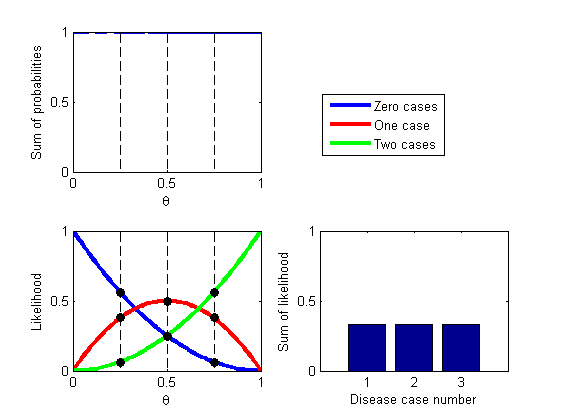
\includegraphics{likelihood_binomial.png}}
\caption{The likelihood function as theta varies for the case of the two possible data. For a fixed value of $\theta$ we find that the sum across the values of the probability is always 1. This is because when viewed in this way, the likelihood is really a discrete probability density across the two values which x can take on. However, when we hold the data fixed (choose either the red or blue line) and sum area under the likelihood curve across the values of $theta$ we do not find that the sum is generally equal to 1. }\label{fig:Likelihood_binomial}
\end{figure}

We will now extend the analysis to cover the case when we have a group of $N$ individuals. Firstly, consider the case when we have a group size of 3. If we assume that the individuals are identically distributed, then the 4 probabilities are of the form:

\begin{equation}\label{eq:Likelihood_binomialThreeProbsSimple}
\begin{align}
P(Z = 0|\theta)& = P(X_1=0,X_2=0,X_3=0|\theta)\\
P(Z = 1|\theta)& = P(X_1=1,X_2=0,X_3=0|\theta)+P(X_1=0,X_2=1,X_3=0|\theta)\\
&  + P(X_1=0,X_2=0,X_3=1|\theta)\\
P(Z = 2|\theta)& = P(X_1=1,X_2=1,X_3=0|\theta) + P(X_1=1,X_2=0,X_3=1|\theta)\\
& + P(X_1=0,X_2=1,X_3=1|\theta)\\
P(Z = 3|\theta)& = P(X_1=1,X_2=1,X_3=1|\theta)
\end{align}
\end{equation}

If we continue to assume independence then we can simplify the probabilities to:

\begin{equation}\label{eq:Likelihood_binomialThreeProbsSimpler}
\begin{align}
P(Z = 0|\theta)& = \;P(X_1=0|\theta) P(X_2=0|\theta)  P(X_3=0|\theta)\\
P(Z = 1|\theta)& = 3P(X_1=1|\theta) P(X_2=0|\theta)  P(X_3=0|\theta)\\
P(Z = 2|\theta)& = 3P(X_1=1|\theta) P(X_2=1|\theta)  P(X_3=0|\theta)\\
P(Z = 3|\theta)& = \;P(X_1=1|\theta)P(X_2=1|\theta) P(X_3=1|\theta)
\end{align}
\end{equation}

Again, we notice a numeric pattern in terms of the first part of each expression $\{1,3,3,1\}$, which happens to correspond exactly to the coefficients on terms for the expansion of $(1+x)^3$. Hence, we can again rewrite the likelihood using the binomial expansion notation:

\begin{equation}\label{eq:Likelihood_binomialThreeFull}
P(Z=\beta|\theta) = {3 \choose \beta} \theta^\beta (1-\theta)^{3-\beta}
\end{equation}

We recognise a pattern in the likelihoods of (\ref{eq:Likelihood_binomialTwoFull}) and (\ref{eq:Likelihood_binomialThreeFull}) which allows us to deduce that, for a sample size of N, that the model likelihood is given by:

\begin{equation}\label{eq:Likelihood_binomialNFull}
P(Z=\beta|\theta) = {N \choose \beta} \theta^\beta (1-\theta)^{N-\beta}
\end{equation}

The likelihood function given in (\ref{eq:Likelihood_binomialNFull}) is known as the binomial probability distribution.

If we had data, then we could test whether the assumptions which we have made are appropriate by calculating the model-implied-probability of this outcome. For example, if we had a sample of 100 people of which 10 had the disease, and we assumed beforehand that the proportion of the population who have the disease is $\theta=1\%$, then we could calculate the probability that we would have achieved a number of cases as bad, or worse than this using the likelihood in \ref{eq:Likelihood_binomialNFull}:

\begin{equation}
P(Z\geq 10|\theta=0.01) = \sum\limits_{Z=10}^{100}{100 \choose Z} 0.01^Z (1-0.01)^{100-Z} = 7.63 \times 10^{-8}
\end{equation}\label{eq:Likelihood_binomialTest}

We have summed over all the disease cases from 10 to 100 here, because we wanted to work out the probability that we would have obtained a result as bad, or worse, than the one which we actually achieved. This is a particular way of carrying out a classical hypothesis test, which we will dispense with later on, but for now it seems a reasonable way of testing our model. 

The probability which we found in this case was extremely small. What does this tell us? Well, it basically says that there is something wrong with our model which we have chosen here. It could be that the actual disease incidence in the population is much higher than the 1\% which we have assumed beforehand. It could also be that our assumption \textit{independence} is violated in this case, for example if we sampled whole households rather than individuals. This could mean that in a particular household, the chance of having the disease, if another member of your family has the disease is substantially higher than that given by the population as a whole. 

It is difficult to gauge what in particular is wrong with our model without knowing further details of data collection as well as how the estimate of 1\% incidence was estimated for the population. However, it does suggest that we need to do adjust one or more of our assumptions, and reformulate the model to take these into account. We should never simply accept that our model is \textit{correct}. A model is only as good as its capability to reproduce the data which we see in real life. In this case we find it is not a good representation, and we should readjust appropriately.

\subsection{The intelligence of a group of people}\label{sec:Likelihood_normal}
Here we are tasked with formulating a model for an intelligence test score for a group of individuals for which we have data. We are told that the test score is on a continuous scale from 0-200. We do not have any information on individual characteristics which might help us to predict scores, although we are going to, for this simplified example, assume that we do know the mean test score $\mu=70$, and its variance $\sigma^2=10$ in the population (although we will relax this assumption in section \ref{sec:Likelihood_MLE}). We might assume that there are a range of factors which overall result in an individual's performance on this test. For example, these might include their schooling, parental education, 'innate' ability, as well as how tired they were feeling on the day of the test. If we assume that there are a large range of such factors and the score which results is an average of all these, then we might assume that the Central Limit Theorem might be appropriate for determining the distribution of test scores. Don't worry if you are not aware of this theorem, we will cover it in due course, but basically it says, if there are a large number of factors\footnote{Technically a infinite number of factors which additively result in the overall score.} which average out to result in an intelligence score, then the normal distribution provides a reasonable approximation to the distribution of test scores. In which case, we might assume that a normal distribution might be reasonable to assume for our likelihood function for an individual's test score, $X$:\\

\begin{equation}
P(X=\alpha|\mu,\sigma^2) &= \frac{1}{\sqrt{2\pi\sigma^2}}e^{-\frac{(\alpha-\mu)^2}{2\sigma^2}}
\end{equation}\label{eq:Likelihood_normal}



\begin{figure}
\centering
\scalebox{0.75} 
{\includegraphics{likelihood_normal.png}}
\caption{A figure with LHS showing a normal distribution with the area to the right of 140 indicated by shading. The RHS shows a normal CDF with the value of 140 indicated.}\label{fig:Likelihood_normal}
\end{figure}

If we obtain an individual within our sample who has achieved a test score of 140, we can ask what is the probability of achieving a result as extreme as this, using our idealised model, by simply integrating the probability density (this is the continuous analogue to the discrete summing that we did in (\ref{eq:Likelihood_binomialTest})):

\begin{equation}
\begin{align}
P(X\geq 140|\mu=70,\sigma^2=10) &= \int\limits_{140}^{\infty}\frac{1}{\sqrt{2\pi\times 10}}e^{-\frac{(\alpha-70)^2}{2\times 10}} \mathrm{d}\alpha\\
 & = 1-\Phi\left(\frac{140-70}{\sqrt{10}}\right) \approx 0
\end{align}\label{eq:Likelihood_normalSampleOne}
\end{equation}

In (\ref{eq:Likelihood_normalSampleOne}), $\Phi$ stands for the value of the \textit{standard} normal cumulative distribution function\footnote{A standard normal has mean 0, and a variance of 1. By taking away the mean of 70, and dividing through by the standard deviation, we transform from an arbitrary mean- and variance-normal, to a \textit{standard} one.} at the value of 140 (see figure \ref{fig:Likelihood_normal} for an explanation). Since we find that the probability of obtaining this data point under our current model is extremely small, we conclude that there is something wrong with our model, and go back to examine the various assumptions that were made in deriving it.

If we also assume that information regarding one individual's test score tells us nothing about another's\footnote{Apart from their joint reliance on $\mu$ and $\sigma^2$.}, then we might assume \textit{independence} for our data. We might also assume that all individuals come from the same population.  These two assumptions - independence and identical distribution - are equivalent to saying that the individually were randomly sampled from the population. We can use these two assumptions to calculate the joint probability density for a sample of N individuals by simply multiplying together the individual densities:


\begin{equation}
P(X_1=\alpha_1,X_2 =\alpha_2,...,X_N=\alpha_N|\mu,\sigma^2) = \prod\limits_{i=1}^{N}\frac{1}{\sqrt{2\pi\sigma^2}}e^{-\frac{(\alpha_i-\mu)^2}{2\sigma^2}}
\end{equation}\label{eq:Likelihood_normalN}


We could then use (\ref{eq:Likelihood_normalN}) to calculate the probability of obtaining a given sample of observations as extreme as the values obtained, again by integrating. However, here it would be slightly more complicated than that of (\ref{eq:Likelihood_normalSampleOne}) since we would have to integrate across all individual's variables. For example if we obtained a sample of $\{75,71\}$ then we could obtain the probability of obtaining a sample as extreme as this under our model:

\begin{equation}
\begin{align}
P(X_1\geq 75,X_2\geq 71|\mu=70,\sigma^2=10) &= \int\limits_{75}^{\infty}\int\limits_{71}^{\infty}\frac{1}{\sqrt{2\pi\times 10}}e^{-\frac{(\alpha_1-70)^2}{2\times 10}}\times e^{-\frac{(\alpha_2-70)^2}{2\times 10}} \mathrm{d}\alpha_1 \mathrm{d}\alpha_2\\
& = \int\limits_{75}^{\infty} \frac{1}{\sqrt{2\pi\times 10}}e^{-\frac{(\alpha_1-70)^2}{2\times 10}} \mathrm{d}\alpha_1  \int\limits_{71}^{\infty} \frac{1}{\sqrt{2\pi\times 10}}e^{-\frac{(\alpha_2-70)^2}{2\times 10}} \mathrm{d}\alpha_2\\
& = (1-\Phi\left(\frac{75-70}{\sqrt(10)}\right))\times (1-\Phi\left(\frac{71-70}{\sqrt(10)}\right)) \approx 0.02
\end{align}
\end{equation}\label{eq:Likelihood_normalSampleN}

In (\ref{eq:Likelihood_normalSampleN}), the integrals are easily separated because we have assumed that the individuals' test scores are independent. If we had not assumed this, then we would have to have done a double integral of a multivariate normal distribution. Again, we have found that it is unlikely that we would have obtained two observations as extreme as this, if our model's assumptions are in fact true. This should prompt us to go back and re-examine these steps.

\section{The subjectivity of model choice}
It is hoped that the analysis in the preceding sections has given us a taste of how we can go about specifying a likelihood for a hitherto unknown circumstance. We start by making assumptions which allow us to simplify the situation, then look for a likelihood which is a good fit to the simplified model, which is then used to test the validity of the assumptions with the sample of data obtained. If the model struggles to explain the data, then we should go back and iteratively modify, then test our model, until it adequately can be thought to represent the real life data obtained.

However, it should be re-emphasised that by its nature, a model is always a simplification of reality. As such, no one model is \textit{correct}. There are often many models that could be used to explain the data which we have to hand. We should always take care to test each of these against its ability to explain the aspect of the data with which we are interested, and only proceed with it if it is adequate in this regard. Real life is complicated, and thus with each of the assumptions that were used to justify a particular model, there will inevitably be a degree of \textit{subjectivity}. As such, no analysis - whether frequentist or Bayesian - can be thought to be purely \textit{objective}. Hence, the human analyst can not, and should not, be replaced by automata for statistical analysis. A degree of subjective judgement is always necessary in statistics, as in all other walks of life.

\section{Maximum likelihood - a short introduction}\label{sec:Likelihood_MLE}
The analysis in section \ref{sec:chooseLikelihood} assumes that we know beforehand the fraction, $\theta$, the populous that are predisposed to having the disease. In reality we rarely know such a thing. Often the main focus of building a statistical model is to try to estimate such parameters from our sample of data to which we have access. A popular frequentist method for achieving this goal is the estimation strategy known as Maximum Likelihood. In this section we will look at how this estimation strategy can yield estimates of parameters, and we will also go on to look at how these estimates can be used to make inferences about what is going on in the population as a whole.

The principal used in Maximum Likelihood estimation is simple. Firstly, we assume a model which we use to approximate the data generating process which resulted in our sample, based on the various assumptions about the real life process which we make. We then calculate what is known as the joint probability of obtaining the sample of observations, assuming that we do not know the parameters which specify completely those distributions. We then choose the parameters which \textit{maximise} the likelihood of obtaining that particular sample of observations. The resultant joint probability distribution gives the highest probability of achieving those observations given this choice of parameters. We will go through some simple examples to illustrate this process. 

\subsection{Estimating disease prevalence}\label{sec:Likelihood_diseaseMLE}
In section \ref{sec:Likelihood_diseaseGroup} we assumed that we knew beforehand the fraction of the population from which our sampled individuals came. As mentioned previously, it is uncommon that such a thing be known before carrying out an analysis. In fact, the reason for undertaking a statistical analysis of the situation is often to try to estimate the underlying prevalence of disease within the population.

If we find that under a sample of 100 individuals, that 10 tested positively (and assuming for simplicity that there are no false-positives), and we make the same assumptions as in section \ref{sec:Likelihood_diseaseGroup} - that of independence and identically-distributed - then we can write down the overall likelihood function using (\ref{eq:Likelihood_binomialNFull}) as:

\begin{equation}\label{eq:Likelihood_binomialNew}
L(\theta|data) = {100 \choose 10} \theta^{10} (1-\theta)^{100-10}
\end{equation}

\begin{figure}
\centering
\scalebox{0.75} 
{\includegraphics{likelihood_logMonotonicity.png}}
\caption{A figure with four panes. The top-left is log-likelihood as a function of likelihood. The bottom-left is likelihood as a function of theta, and log-likelihood plotted on the same axis. Top-right is a weird function of likelihood as a function of likelihood. Below it a graph of likelihood as a function of theta, with a different maximum reached for the weird function.}\label{fig:Likelihood_logMonotonicity}
\end{figure}

Remember, that since we are varying $\theta$ and holding the data constant here, that (\ref{eq:Likelihood_binomialNew}) is a \textit{likelihood}, not a probability. We then need to simply choose $\theta$ so that we can maximise the likelihood. We could simply differentiate (\ref{eq:Likelihood_binomialNew}) as it stands, and set the derivative equal to 0; rearranging the resultant equation for $\theta$. However, to make life a little easier for us, we are first going to take the \textit{log} of this expression, then differentiate it, setting the derivative to 0; resulting in the same value of $\theta$. We are able to do this because of the simple properties of the log transformation (see figure \ref{fig:Likelihood_logMonotonicity}):

\begin{equation}\label{eq:Likelihood_logLikelihoodBinomial}
l(\theta|data) = log{100 \choose 10}+ 10log(\theta)+ 90 log(1-\theta)
\end{equation}

Where to get the result (\ref{eq:Likelihood_logLikelihoodBinomial}), we have used the log rules:

\begin{equation}\label{eq:Likelihood_logRules}
\begin{align}
log(ab) &= log(a) + log(b)\\
log(a^b) &= blog(a)
\end{align}
\end{equation}

We can now simply differentiate the log-likelihood $l(\theta|data)$:

\begin{equation}\label{eq:Likelihood_binomialderiv}
\frac{\partial l}{\partial \theta} = \frac{10}{\hat{\theta}}-\frac{90}{1-\hat{\theta}} = 0
\end{equation}

If we set the derivative to 0 we then obtain the maximum likelihood \textit{estimator}, $\hat{\theta} = \frac{1}{10}$ (see figure \ref{fig:Likelihood_MLE}). We have placed hats on $\theta$ to emphasise that this is an estimator for the variable. An estimator is a mathematical function which outputs an estimate of a parameter in our model.

\begin{figure}
\centering
\scalebox{0.75} 
{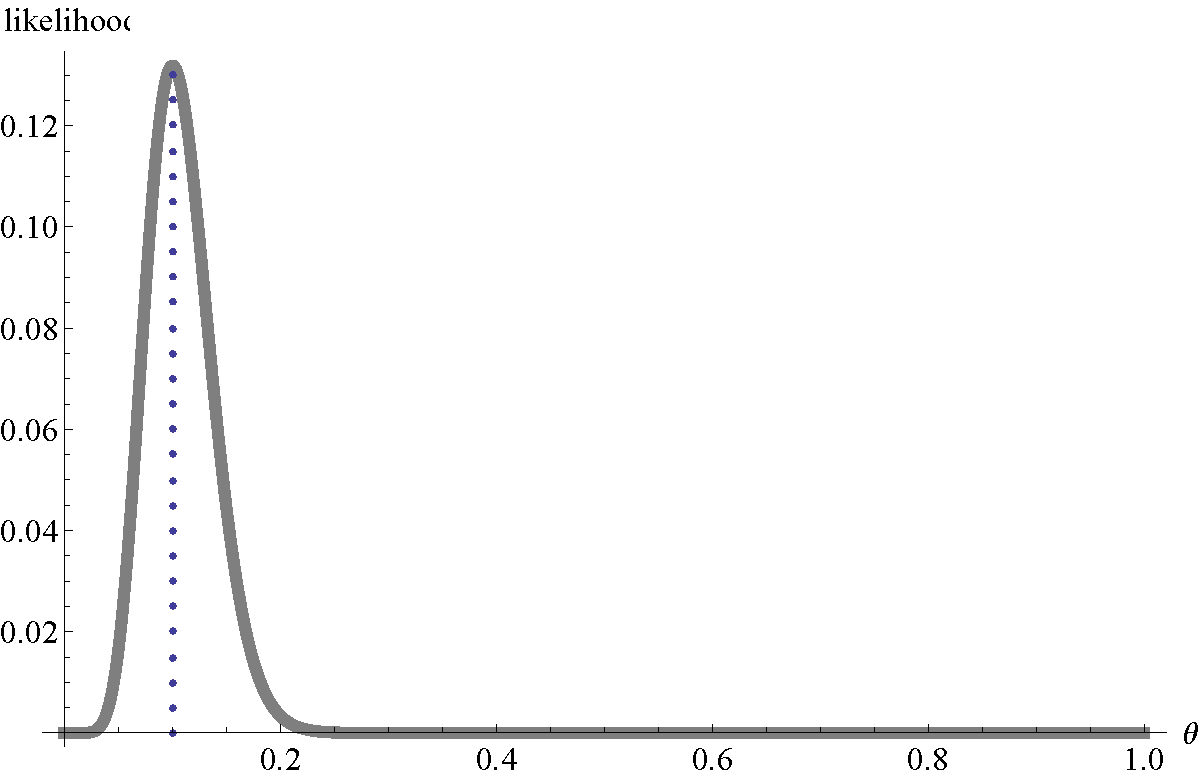
\includegraphics{Likelihood_ML.png}}
\caption{A figure displaying log-likelihood as a function of theta, maximised at 1/10.}\label{fig:Likelihood_MLE}
\end{figure}


This estimator makes sense intuitively. The value of the parameter which results in the highest likelihood of obtaining the data occurs when the population prevalence exactly matches that obtained in our sample. In general if we found a number $\beta$ of individuals out of a sample of size $N$, who were disease-positive, then we would again find that the preceding analysis results in an estimator of the disease prevalence exactly equal to that in our sample:

\begin{equation}\label{eq:Likelihood_binomialestimator}
\hat{\theta} = \frac{\beta}{N}
\end{equation}

\subsection{Estimating the mean and variance in intelligence scores}
We are given a sample of individuals with test scores $\{75,71\}$, and we model the test scores using a normal likelihood as described in section \ref{sec:Likelihood_normal}:

\begin{equation}\label{eq:Likelihood_normalTwo}
L(\mu,\sigma^2|X_1=75,X_2 =71) = \frac{1}{\sqrt{2\pi\sigma^2}}e^{-\frac{(75-\mu)^2}{2\sigma^2}}\times \frac{1}{\sqrt{2\pi\sigma^2}}e^{-\frac{(71-\mu)^2}{2\sigma^2}}
\end{equation}

We can then proceed as we did in section \ref{sec:Likelihood_diseaseMLE} by taking the log of this expression before we differentiate it:

\begin{equation}\label{eq:Likelihood_diseaseLogLikelihood}
l(\mu,\sigma^2|X_1=75,X_2 =71) = 2log\left(\frac{1}{\sqrt{2\pi\sigma^2}}\right)-{\frac{(75-\mu)^2}{2\sigma^2}}-{\frac{(71-\mu)^2}{2\sigma^2}}
\end{equation}

Where we have again used the log rules in (\ref{eq:Likelihood_logRules}) to achieve (\ref{eq:Likelihood_normalTwo}). We can now proceed to differentiate (\ref{eq:Likelihood_diseaseLogLikelihood}) with respect to both variables, holding the other constant, setting each to 0, to achieve the following:

\begin{equation}\label{eq:Likelihood_diseaseDerivativeOne}
\begin{align}
\frac{\partial l}{\partial \mu} &= {\frac{(75-\hat{\mu})}{\hat{\sigma^2}}}+{\frac{(71-\hat{\mu})}{\hat{\sigma^2}}} = 0\\
\frac{\partial l}{\partial \sigma^2} &= -\frac{1}{\hat{\sigma^2}} + \frac{(75-\hat{\mu})^2+(71-\hat{\mu})^2}{2\hat{\sigma^4}} = 0
\end{align}
\end{equation}

The first of these expressions yields $\hat{\mu} = \frac{71+75}{2} = 73$, which when put into the second gives: 

\begin{equation}
\hat{\sigma^2} = \frac{1}{2}\left[(75-73)^2 + (71-73)^2)\right] = 4
\end{equation}

Notice that the maximum likelihood estimators for the population mean and variance are for this case the \textit{sample mean} and \textit{sample variance}\footnote{Albeit a biased estimator of the population variance. The unbiased estimator would divide by 1.}. In fact, this holds for the case of N individuals' data, then the maximum likelihood estimators for this case would be:

\begin{equation}
\hat{\sigma^2} = \frac{1}{N}\sum\limits_{i=1}^{N} X_i = \bar{X}
\end{equation}
\begin{equation}
\hat{\sigma^2} = \frac{1}{N}\sum\limits_{i=1}^{N}(X_i-\bar{X})^2 = s^2
\end{equation}

\section{Frequentist inference in Maximum Likelihood}
We have now detailed how to derive point estimates of parameters using the method of maximum likelihood. However, at the moment we are unable to make any conclusions about the population. This is because we do not have any idea as to whether we obtained a particular estimate of a parameter due to picking a weird sample, or because it \textit{actually} has a value in the population which is at this value. Frequentists get round this by examining a graph of log-likelihood near the maximum likelihood point estimate (see figure \ref{fig:Likelihood_likelihoodCurvature}). If the log-likelihood is strongly peaked near the maximum likelihood estimate, then this suggests that only a small range of parameters would yield a likelihood near the ML value. By contrast, if the log-likelihood is gently peaked near the ML estimate, then it is feasible that a large range of parameters would yield estimates close to this value. In the latter case, it seems logical that we should be less confident in the particular value of the parameter which is given by maximum likelihood. We can measure the 'peakedness' in the log-likelihood by looking at the magnitude of the second derivative\footnote{The first derivative gives the gradient, the second derivative gives the rate of change of the gradient - a measure of curvature.} of the function at the ML point estimate value. The more curved the log-likelihood, the more confident we can be of our estimated parameter value, and the more certain we can be about making conclusions on the population. Note however, that the frequentist inference is not based on proper probability distributions (since we infer based on a likelihood). This contrasts with the Bayesian method which, by its nature, allows for a more complete description of parameters, and thus a less opaque manor in which to draw inferences.

\section{Chapter summary}
We should now understand what is meant by a likelihood, and how to build probabilistic models of real life processes. Of course, the difficulty of modelling a process is governed by its degree of complexity and sensitivity to violations of assumptions. Further we should also understand how the frequentist method of Maximum Likelihood can be used to yield point estimates of parameters. We are however, currently restricted in our ability to make inferences based on full probability distributions over parameters. Bayes' rule tells us how we can convert from a likelihood - itself not a proper probability distribution - to a posterior (\textit{correct}) probability distribution for parameters. In order to use to do this though, we need to understand what is meant by a \textit{prior} distribution and how we can specify this distribution to suit the particular situation. This is what is covered in the next chapter.

\chapter{Priors}
\section{Chapter Mission statement}
At the end of this chapter a reader will know what is meant by a prior, and the different philosophies that are used to construct and understand them. 

Insert a graphic with the likelihood part of Bayes' formula circled, as in the equation shown below for the part highlighted in blue.

\begin{equation}
P(\theta|data) = \frac{P(data|\theta)\times {\color{blue}P(\theta)}}{P(data)}
\end{equation}\label{eq:Prior_BayesHighlighted}

\section{Chapter goals}
Bayes' rule tells us how to convert a likelihood - itself not a proper probability distribution - into a posterior probability distribution for parameters, which can then be used for inference. The likelihood tells us what the data implies are most likely values of the parameters, but without a prior weighting of the probability of each of these parameter values, it is not that useful. Bayesian analysis requires that we specify this pre-data weighting ascribed to different parameter values in a full probability distribution which is known as a \textit{prior}. Priors are without doubt the most controversial aspect of Bayesian statistics, with its opponents criticising its inherent \textit{subjectivity}. It is hoped that by the end of the chapter we will have convinced the reader that, not only is subjectivity inherent in \textit{all} statistical models - both frequentist and Bayesian - but the explicit subjectivity of priors is more transparent, and hence open to interrogation, than the implicit subjectivity abound elsewhere.

This chapter will also explain the differing interpretations which are ascribed to priors. The reader will come to understand the types of method that can be used to construct prior distributions, and how they can be chosen to be minimally subjective or less so. Finally, the reader will understand that if significant data are available then the conclusions drawn should be insensitive to the initial choice of prior.

\section{What are priors, and what do they represent?}
Two representations of a prior. The data converts our prior knowledge in a logical way to a posterior distribution. Alternatively, the prior tells us how to convert the likelihood into a proper probability distribution.

Chapter \ref{chap:Likelihoods} introduced us to the concept of formulating a likelihood, and how this can be used to derive frequentist estimates of parameters, using the method of maximum likelihood. This pre-supposes that the parameters in question are immutable, fixed quantities that actually exist, and can be estimated by methods that can be repeated, or imagined to be repeated many times \cite{gill2007bayesian}. As Gill (2007) indicates, this is unrealistic for the vast majority of social science research.

\begin{quotation}
It is simply not possible to rerun elections, repeat surveys under exactly the same conditions, replay the stock market with exactly matching market forces, or re-expose clinical subjects to identical stimuli.
\end{quotation}

For Bayesians, it is the data that are treated as fixed, and the parameters that vary. The likelihood is then combined with the prior distribution, in the numerator of Bayes' rule to help us to deduce the post-data distribution of the parameter in question. But what does it actually mean for a parameter to have a prior distribution?

Gelman et al. (2013) suggests that there are two different interpretations of priors: the \textit{population} interpretation where the current value of a parameter is the result of a draw from a true population distribution; alternatively, in the more subjective \textit{state of knowledge} interpretation, we specify our knowledge and uncertainty in a parameter as if regarding it as a draw from a probability distribution \cite{gelman2013bayesian}.

\section{Why don't we just normalise likelihood by choosing a unity prior?}
Why can't be simply let the prior be unity for all values of $\theta$, in other words set $P(\theta) = 1$ in the numerator of Bayes' rule; resulting in a posterior that takes the form of a normalised likelihood:

\begin{equation}
P(\theta|data) = \frac{P(data|\theta)} {P(data)}
\end{equation}\label{eq:Prior_BayesNormalisedLikelihood}


This would surely negate the need for specification of a prior, and thwart all attempts to denounce Bayesian statistics as \textit{subjective}. So won't don't we do just that? 

It is hoped that 


\section{The explicit subjectivity of priors}
\section{An urn of balls} 
Bayes' box from Bolstad.
\section{Disease proportions revisited}
\section{Constructing priors}
\subsection{Vague priors}
\subsection{Informative priors}
\subsection{Conjugate priors}
\subsection{Eliciting priors}
Gill example. x and z.
\section{A strong model is independent of priors}
\section{Chapter summary}



\bibliographystyle{plain}
\bibliography{Bayes}

\end{document}